\section{Introducción}
\label{sec:introduccion}
La fibra óptica constituye un medio fundamental para las redes de telecomunicaciones: se utiliza en enlaces de transporte, en conexiones punto a punto y en redes de acceso FTTH (\textit{Fiber to the Home}, fibra hasta el hogar). Las redes FTTH con tecnología GPON permiten brindar acceso a Internet, telefonía, televisión y otros servicios mediante una infraestructura óptica compartida, cuyo diseño requiere integrar criterios de cobertura, capacidad, distribución de fibras, selección de componentes y presupuesto óptico.

En este trabajo se desarrolla una propuesta de red FTTH GPON para la localidad de Marcos Juárez, provincia de Córdoba, tomando como referencia el área de cobertura indicada por la cátedra (\autoref{fig:area_cobertura}). El nodo cabecera se ubica en la Cooperativa COYSPU (9 de Julio 99-149) y el área se divide en las regiones Este y Oeste según la traza de la Ruta Nacional 12.

\begin{figure}[H]
    \centering
    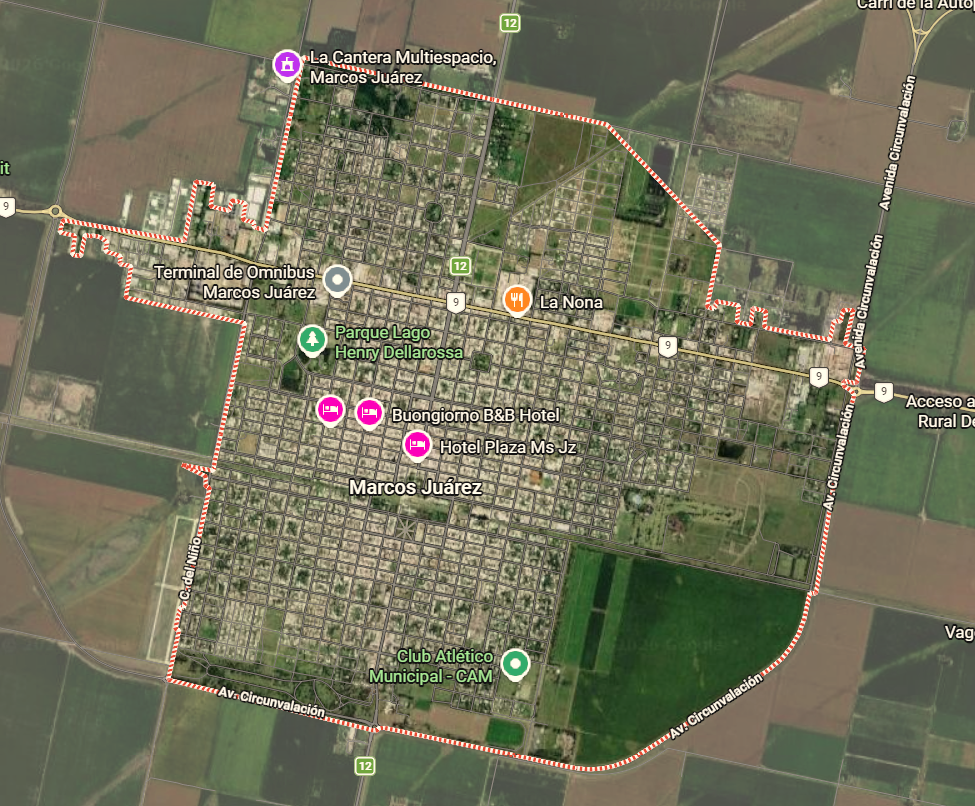
\includegraphics[width=0.85\textwidth]{area_cobertura.png}
    \caption{Área de cobertura de la red en la localidad de Marcos Juárez. Fuente: consigna de la cátedra.}
    \label{fig:area_cobertura}
\end{figure}

\pendiente{describir la organización del informe una vez completadas las secciones.}
